\documentclass[10pt,]{beamer}

\newcommand{\lectnum}{L16}
\newcommand{\lecttitle}{Mixtures of Experts\\Crowdsourcing}

\usepackage{amsmath, amssymb, graphicx}
\usepackage[]{algorithm2e}
\usepackage{pdfpages}
\usepackage[british]{babel}

\hypersetup{colorlinks,linkcolor=,urlcolor=blue}
\newenvironment{titledslide}[1]{\begin{frame}\frametitle{#1}}{\end{frame}}

\mode<presentation>{\setbeamercovered{transparent}}

\setbeamertemplate{sidebar right}{}
\setbeamertemplate{footline}{%
\hfill\usebeamertemplate***{navigation symbols}
\hspace{0.4cm}\lectnum: \insertframenumber{}/\inserttotalframenumber \hspace*{0.4cm}}

\author{James Cussens}

\title{COMS30035, Machine learning:\\ \vspace{5pt} \lecttitle}

\institute{School of Computer Science\\University of Bristol}

\begin{document}
%%%%%%%%%%%%%%%%%%%%%%%%%%%%%%%%%%%%%%%%%%%%%%%%%%%%%%%%%%%%%%%%%%%%%%

\begin{frame}
  \titlepage
\end{frame}

%%%%%%%%%%%%%%%%%%%%%%%%%%%%%%%%%%%%%%%%%%%%%%%%%%%%%%%%%%%%%%%%%%%%%%



%%%%%%%%%%%%%%%%%%%%%%%%%%%%%%%%%%%%%%%%%%%%%%%%%%%%%%%%%%%%%%%%%%%%%%
\begin{titledslide}{Acknowledgement}

  \begin{itemize}
  \item These slides are adapted from ones originally created by Edwin Simpson. 
  \end{itemize}
  
\end{titledslide}

\begin{frame}[fragile]
\frametitle{Agenda}   % expectation: 33 slides + title and agenda, 11 slides per chunk
\begin{itemize}
\item \textcolor{gray}{Model Selection
\item Model Averaging
\item Ensembles: Bagging
\item Ensembles: Boosting and Stacking
\item Tree-based Models % decision trees effectively make the selection decisions on the fly; random forests then are ensembles. Maybe trees should be discussed before committees?
\item Conditional Mixture Models}  % this may be in the next "lecture"?
\item Ensembles of Humans  
\end{itemize}
\end{frame}



\begin{frame}
\frametitle{Wisdom of the crowd}
\begin{itemize}
\item Remember the equation relating the error of a combination to the error of an average individual: $E_{COM} = \frac{1}{M} E_{AV}$ 
\item Assuming uncorrelated, zero-mean errors
\item Can we apply this when the base models are people rather than machine learners?
\item Could combinations of humans be used in machine learning? 
%In this case we have the \emph{wisdom of the crowd} -- the average guess from a crowd of people is often surprisingly accurate
\end{itemize}
%In 1907, Sir Francis Galton asked 787 villagers to guess the weight of an ox. None of them got the right answer, but when Galton averaged their guesses, he arrived at a near perfect estimate

\centering
\includegraphics[scale=0.7]{../figures/crowd}
\includegraphics[scale=0.05]{../figures/Musk_ox}
\end{frame}


\begin{frame}
\frametitle{Dataset Annotation}
\begin{itemize}
\item Annotation of datasets is extremely important for machine learning and scientific data analysis:
\begin{itemize}
\item E.g., training labels for supervised learning
\item E.g., test labels for evaluation
\item Where do these annotations come from? 
\uncover<2->{\item In a huge range of applications, somebody has to label the data manually (text, images, biological data, astronomy,...). }
\end{itemize}
% unless the true label is obtained directly from a physical measurement or sensor reading
\centering
\includegraphics[scale=0.033]{../figures/galaxy}
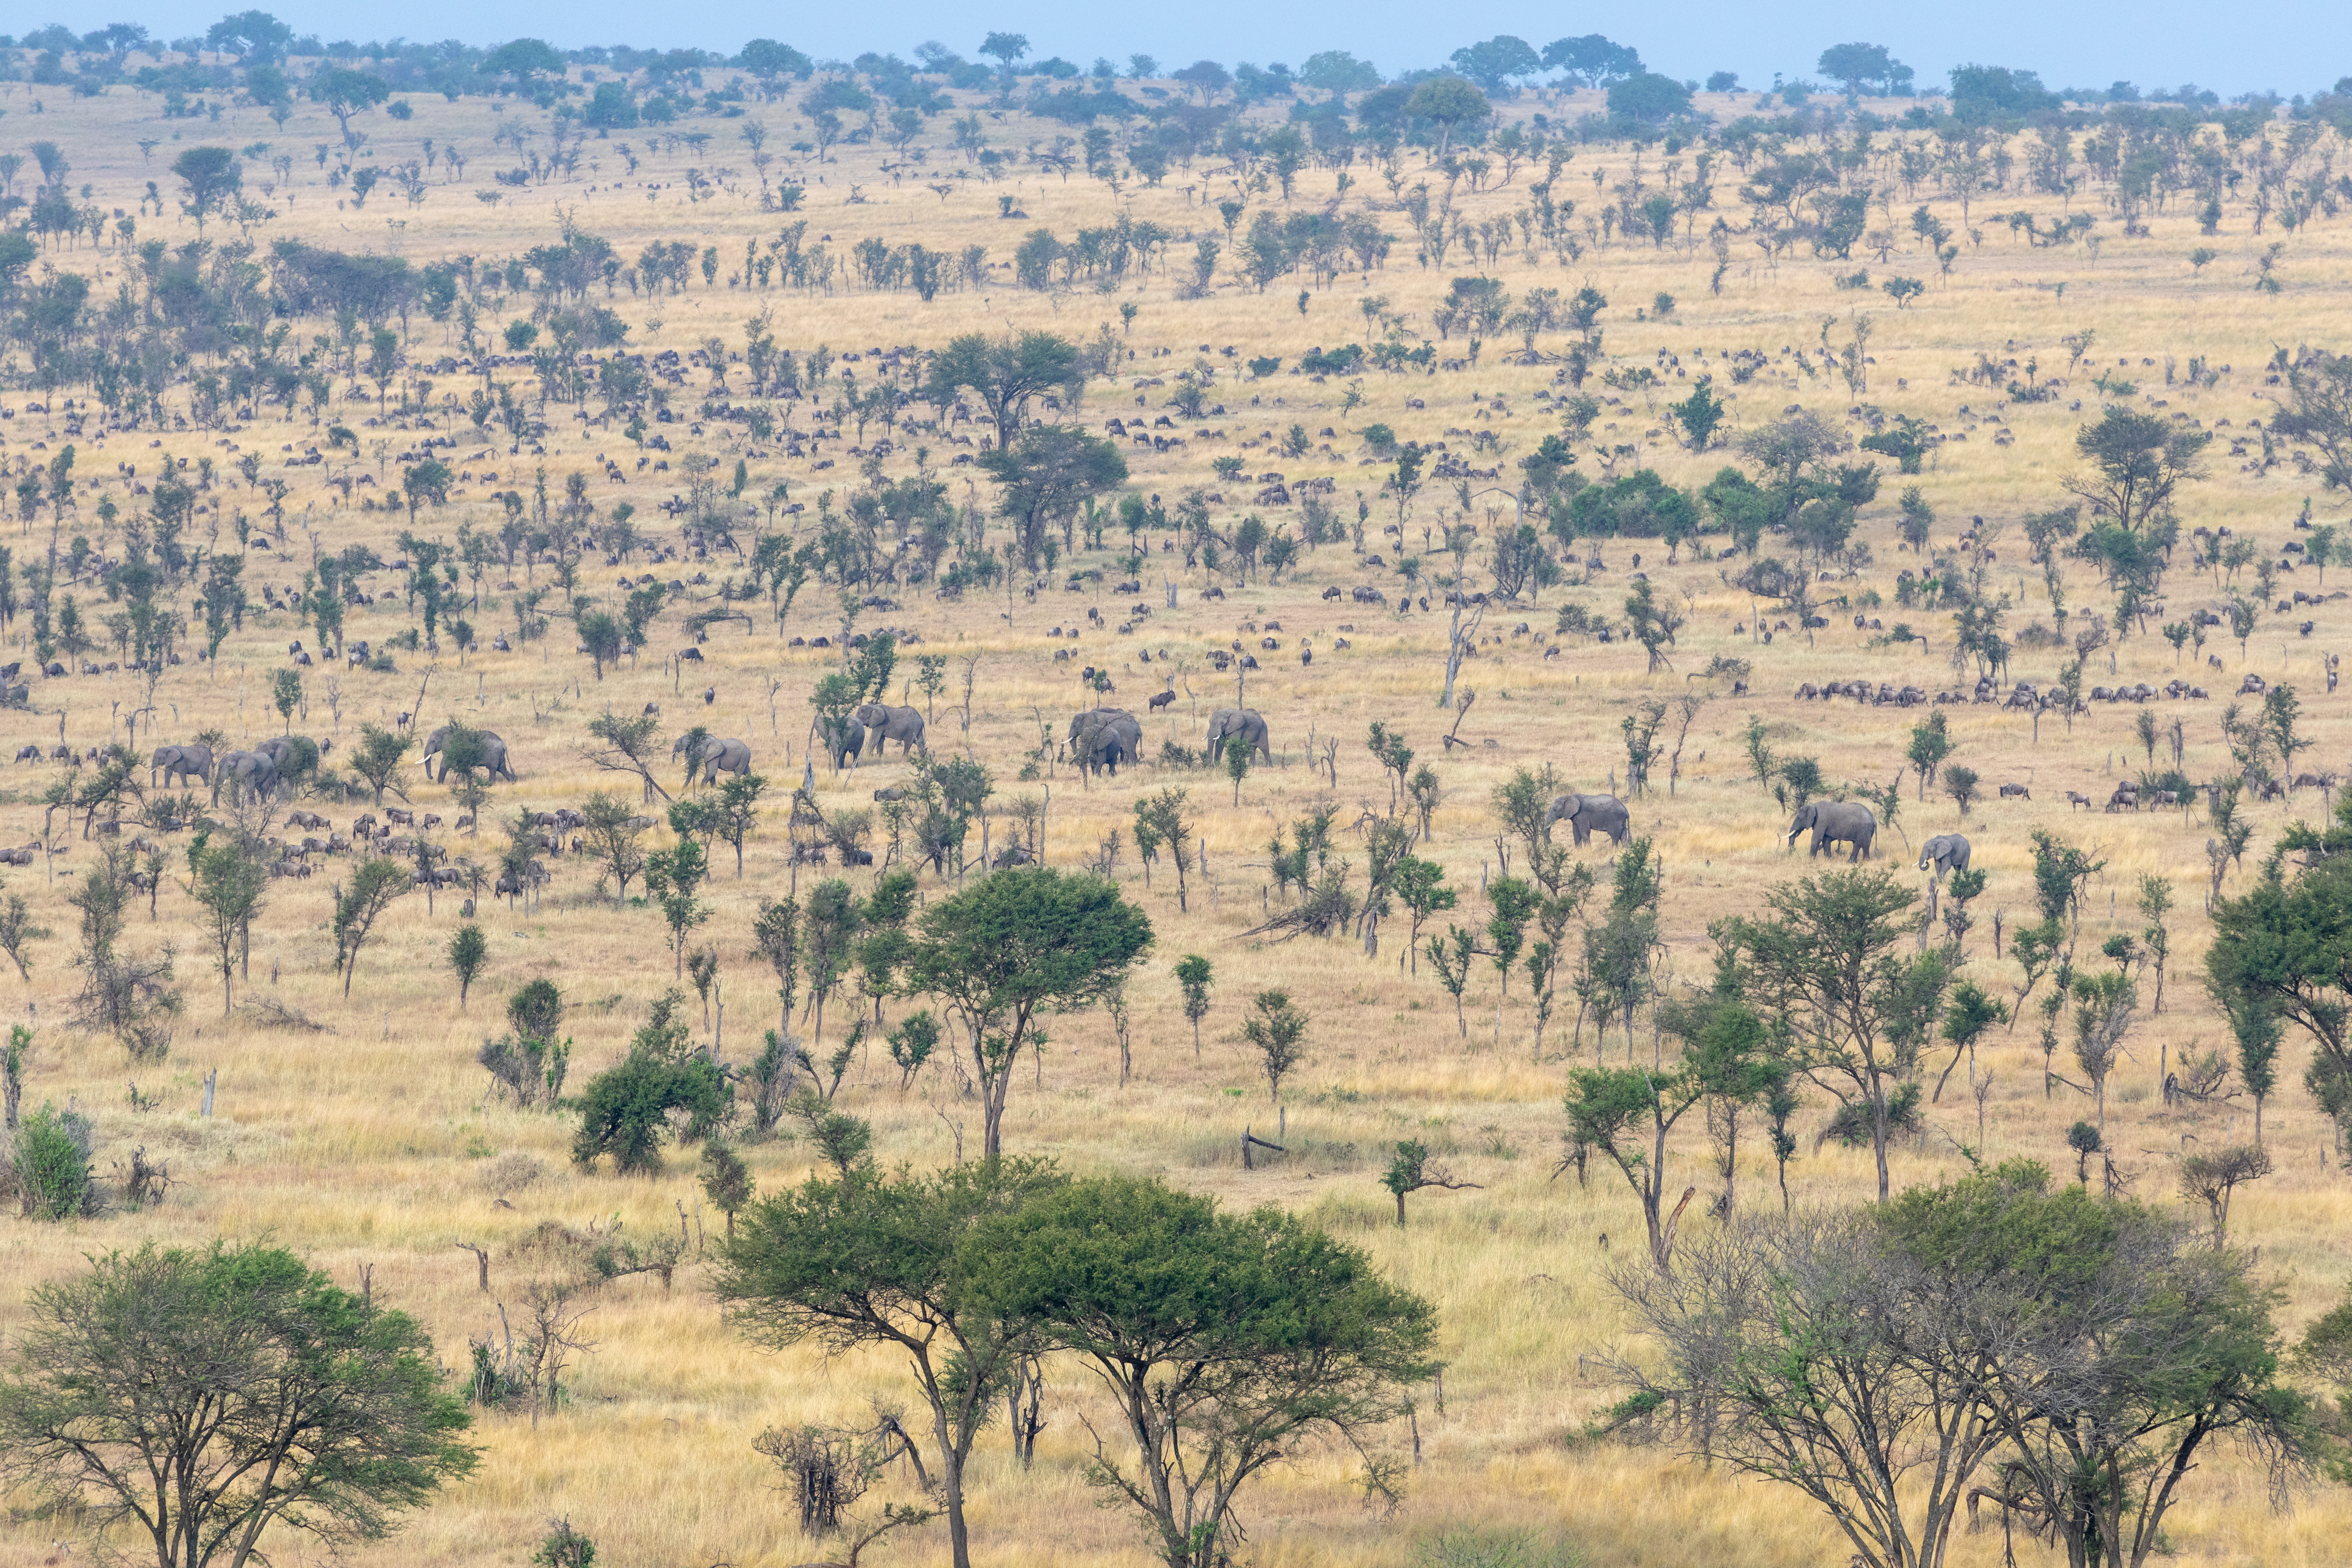
\includegraphics[scale=0.05]{../figures/serengeti}
%\item Why is this relevant to machine learning?
\uncover<3->{\item There are many tasks that people can do that computers cannot, even though we make many errors.
\begin{itemize}
\item E.g., following instructions
\item E.g., applying commonsense reasoning
\end{itemize}}
\end{itemize}
\end{frame}


\begin{frame}
\frametitle{Expert Annotators}
\begin{itemize}
\item Expert annotators have a low average error, $E_{AV}$
\item People make mistakes, even experts, so combine multiple annotations from different people.
\item We would like to collect large datasets to support more extensive testing and more complex models
\item Experts' time is expensive and limited, so how can we obtain large datasets at reasonable speed and cost?
\uncover<2->{\item This is where the wisdom of the crowd comes in!}
\end{itemize}
\end{frame}


\begin{frame}
\frametitle{Crowdsourcing}
\begin{itemize}
\item Ask a large number of non-expert annotators to provide the data!
\item Crowdsourcing platforms allow \emph{requesters} to create  
tasks for \emph{crowd workers}
\uncover<2->{\item Amazon Mechanical Turk -- pay a few cents per task }
\uncover<3->{\item Zooniverse -- volunteer citizen scientists }
\end{itemize}
\uncover<2->{\includegraphics[scale=0.5]{../figures/amt}}
\uncover<3->{\includegraphics[scale=0.16]{../figures/zooniverse_projects}}
\end{frame}


\begin{frame}
\frametitle{A Crowdsourcing Task}
\begin{itemize}
\item Tasks need to be simple with clear instructions
\item See http://www.zooniverse.org for many more
\end{itemize}
\centering
\includegraphics[scale=0.25]{../figures/galaxy_zoo}
\end{frame}


\begin{frame}
\frametitle{Crowd Size vs. Error Rate}
\begin{itemize}
\item Crowdsourced annotations have lower quality, higher $E_{AV}$
\item What can we do about this?
\uncover<2->{\item Remember $E_{COM} = \frac{1}{M} E_{AV}$:
\item We can prevent  $E_{COM}$ from rising by increasing $M$.
\item So, using a larger number of crowd annotators  allows us to obtain quality annotations at far reduced costs.}
\end{itemize}
\end{frame}


\begin{frame}
\frametitle{Example: Cheap and Fast -- But Is It Good?} 
\begin{columns}
\column{0.5\textwidth}
\begin{itemize}
\item Systematic comparison of workers to experts on various NLP tasks
\item E.g. rate headlines to reflect emotional content
\uncover<2->{\item Y-axis: correlation with mean of experts
\item Green dashed lines: 1 expert
\item Black solid lines: increasing number of workers per task
\uncover<3->{\item On average, 4 workers compares to 1 expert }}
\end{itemize}
\column{0.5\textwidth}
\uncover<2->{\includegraphics[scale=0.45]{../figures/cheap_but}}
\end{columns}

{\tiny Rion Snow, Brendan O'Connor, Daniel Jurafsky, and Andrew Y. Ng. 2008. \emph{Cheap and fast - but is it good?: evaluating non-expert annotations for natural language tasks} (EMNLP-08).
}
\end{frame}


\begin{frame}
\frametitle{Caveats}
\begin{itemize}
\item Errors are not zero-mean and uncorrelated in practice.
\item The design of the task, the way the data is presented to the crowd, 
the instructions and lack of expertise may mean that most annotators make the same mistakes.
\item There are also spammers who don't make an effort to provide correct labels
\item Annotators have different levels of skill
\end{itemize}
\end{frame}


\begin{frame}
\frametitle{Remedies}
\begin{itemize}
\item Correlated errors are tricky to deal with
\item Address spamming and skill levels by learning a weighted combination function
\item Similar to the \emph{stacking} approach for ensembles of machine learners
\item But not all annotators label all data points...
\item Use the generative model for combining classifiers proposed by Dawid and Skene in 1979
%interpretable
%works well with small amounts of data for each annotator
%missing labels from annotators
\end{itemize}

\tiny Dawid, A. P., \& Skene, A.  M. (1979). Maximum likelihood estimation of observer error-rates using the EM algorithm. Journal of the Royal Statistical Society: Series C (Applied Statistics), 28(1), 20-28.
\end{frame}


\begin{frame}
\frametitle{Dawid and Skene (1979)}
\begin{itemize}
\item For each data point, each annotator $k$ produces label $c^{(k)}$ from $\{1,...,J\}$.
\item To predict the true label $t$ given a set of noisy annotations $\bs c$:
\begin{equation}
p(t=j | \bs c) = \frac{p(t=j)\prod_{k=1}^K\ p(c^{(k)} | t=j) }{\sum_{l=1}^J \left\{ 
p(t=l) \prod_{k=1}^K p(c^{(k)} | t=l) \right\} }.
\end{equation}
\end{itemize}
\centering
\end{frame}


\begin{frame}
\frametitle{Dawid and Skene (1979)}
\begin{itemize}
\item Each annotator is modelled by a confusion matrix, $\bs\pi^{(k)}$ where each entry is $ \pi_{ji}^{(k)} = p(c^{(k)} = i | t=j)$.
\item $\bs\pi^{(k)}$ captures the annotator's different error rates for each class label.
\item Can learn $\pi^{(k)}$ with EM, but Bayesian inference is more effective since the amount of data for many annotators is very small.
\end{itemize}
\centering
\includegraphics[scale=0.45]{../figures/conf_mat}
\end{frame}


\begin{frame}
\frametitle{Example of Dawid and Skene (simulated data)}  % plot comparing ibcc or ds to mv
\centering
Combining noisy classifications using majority vote vs Bayesian treatment of Dawid \& Skene's model (IBCC). 

\includegraphics[scale=0.6]{../figures/mv_ibcc}
\end{frame}


\begin{frame}
\frametitle{Summary}
\begin{itemize}
\item We can also combine people as well as machines using the same model combination principles.
\item Combining lots of human annotators helps do tasks that machine learners can't do, such as constructing training and evaluation datasets.
\item The Dawid and Skene model helps account for different skill levels and down-weight spammers and can be applied as a stacking approach to ensembles of machine learners.
\end{itemize}
\end{frame}

\begin{titledslide}{Reading}

  \begin{itemize}
  \item None!
  \end{itemize}
  
  
\end{titledslide}
%%%%%%%%%%%%%%%%%%%%%%%%%%%%%%%%%%%%%%%%%%%%%%%%%%%%%%%%%%%%%%%%%%%%%%
\begin{titledslide}{Problems and quizzes}

  \begin{itemize}
  \item No problems.
  \item Quizzes:
    \begin{itemize}
    \item Week~8: Ensembles of Humans
    \end{itemize}
  \end{itemize}
  
\end{titledslide}
%%%%%%%%%%%%%%%%%%%%%%%%%%%%%%%%%%%%%%%%%%%%%%%%%%%%%%%%%%%%%%%%%%%%%%
\bibliographystyle{alpha}
\bibliography{../ml}




\end{document}
